% evaluation.tex

%%%%%%%%%%%%%%%%%%%%
\begin{frame}{Experimental Evaluation}
	\begin{center}
		\begin{enumerate}[(1)]
			\setlength{\itemsep}{15pt}
			\item \red{\it Effective:}
			  Can \polysi{} find SI violations in production databases?
			\item \blue{\it Informative:}
			  Can \polysi{} provide understandable counterexamples for SI violations?
			\item \purple{\it Efficient:}
			  How efficient is \polysi?
		\end{enumerate}

		% \vspace{0.50cm}
		% \url{https://github.com/hengxin/PolySI-PVLDB2023-Artifacts}
	\end{center}
\end{frame}
%%%%%%%%%%%%%%%%%%%%

%%%%%%%%%%%%%%%%%%%%
\begin{frame}{Workloads}
	\begin{center}
		{% workload.tex

\begin{table}[t]
  \centering
  \caption{Workload parameters and their default values.\footnote{
		Use a database schema of a \blue{\it two-column table} storing keys and values.
  }}
  \label{param-defaults}
	\renewcommand\arraystretch{1.2}
	\resizebox{0.50\textwidth}{!}{
    \begin{tabular}{|c||c|}
    \hline
    Parameter   & Default Value \\ \hline \hline
    \#sess      & 20   \\ \hline
    \#txns/sess & 100  \\ \hline
    \#ops/txn   & 15   \\ \hline
    \#keys      & 10, 000  \\ \hline
    \%reads     & 50\% \\ \hline
	  distribution    & zipfian \\ \hline
 \end{tabular}}
\end{table}}
	\end{center}
\end{frame}
%%%%%%%%%%%%%%%%%%%%

%%%%%%%%%%%%%%%%%%%%
\begin{frame}{Benchmarks}
	\begin{center}
		\begin{description}[GeneralRW:]
			\setlength{\itemsep}{10pt}
			\item[RuBiS:] an eBay-like bidding system
			\item[TPC-C:] an open standard for OLTP benchmarking
			\item[C-Twitter:] a Twitter clone
			\vspace{10pt}
			\item[GeneralRH:] read-heavy workloads with $95\%$ reads
			\item[GeneralRW:] medium workloads with $50\%$ reads
			\item[GeneralWH:] write-heavy workloads with $30\%$ reads
		\end{description}
	\end{center}
\end{frame}
%%%%%%%%%%%%%%%%%%%%

%%%%%%%%%%%%%%%%%%%%
\begin{frame}{Reproducing Known SI Violations}
	\begin{center}
		{% effectiveness-reproduce.tex

\begin{table}[t]
  \centering
  \caption{Reproducing known SI violations.}
	\renewcommand\arraystretch{1.5}
  \resizebox{0.70\textwidth}{!}{
	\begin{tabular}{cccl}
    \hline
    {\bf Database} & {\bf GitHub Stars} & {\bf Kind} & {\bf Release} \\ \hline
    CockroachDB &	25.1k  &  Relational & v2.1.0, v2.1.6 \\ % \cite{Cobra:OSDI2020} \\
 %   Fauna &	650 &  Document & v2.5.4 \\% \cite{Cobra:OSDI2020} \\
    MySQL-Galera &	381  &  Relational & v25.3.26 \\%\cite{Complexity:OOPSLA2019}\\
    YugabyteDB & 6.7k	 &  Multi-model & v1.1.10.0 \\% \cite{Cobra:OSDI2020}  \\
	  \hline
\end{tabular}}
\end{table}}
		\vspace{0.80cm}

		An extensive collection of 2477 anomalous histories \\[2pt]
		\ncite{Complexity:OOPSLA2019, CockroachDB-bug, YugabyteDB-bug}
	\end{center}
\end{frame}
%%%%%%%%%%%%%%%%%%%%

%%%%%%%%%%%%%%%%%%%%
\begin{frame}{Detecting New SI Violations}
	\begin{center}
		\red{Dgraph}: helped the Dgraph team \blue{confirm} some of their suspicions
		  about their latest release

		\vspace{0.50cm}
		{% effectiveness-new.tex

\begin{table}[t]
  \centering
  \caption{Detecting new violations.}
	\renewcommand\arraystretch{1.5}
  \resizebox{0.85\textwidth}{!}{
	\begin{tabular}{cccl}
    \hline
    {\bf Database} & {\bf GitHub Stars} & {\bf Kind} & {\bf Release} \\ \hline
    Dgraph & 18.2k &  Graph & v21.12.0 \\
    MariaDB-Galera & 4.4k &  Relational & v10.7.3 \\
    YugabyteDB & 6.7k &  Multi-model & v2.11.1.0 \\
    \hline
\end{tabular}}
\end{table}}
		\vspace{0.50cm}

		\red{Galera}: \blue{confirmed} the incorrect claim on preventing ``lost updates''
		  for transactions issued on different cluster nodes
	\end{center}
\end{frame}
%%%%%%%%%%%%%%%%%%%%

%%%%%%%%%%%%%%%%%%%%
\begin{frame}{Understanding Violations (Lost Update)}
	\begin{center}
		% informativeness.tex

\begin{figure}[t]
  \centering
    \begin{subfigure}[b]{0.40\textwidth}
        \centering
        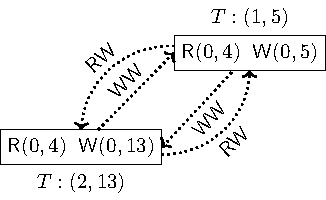
\includegraphics[width = \textwidth]{figs/galera-original}
        \caption{Original output}
    \end{subfigure}\hspace{3ex} \pause
    \begin{subfigure}[b]{0.40\textwidth}
        \centering
        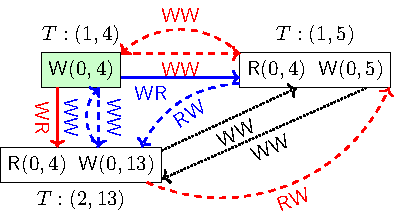
\includegraphics[width = \textwidth]{figs/galera-recovery-1}
        \caption{Missing  participants}
    \end{subfigure}\hspace{3ex} \pause
    \begin{subfigure}[b]{0.40\textwidth}
        \centering
        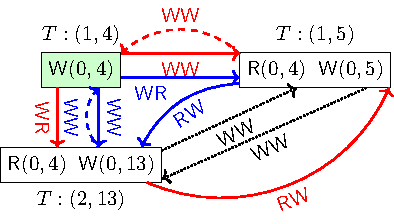
\includegraphics[width = \textwidth]{figs/galera-recovery-2}
        \caption{Recovered scenario}
    \end{subfigure}\hspace{3ex} \pause
    \begin{subfigure}[b]{0.40\textwidth}
        \centering
        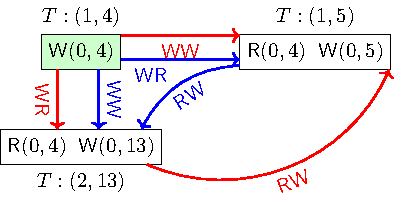
\includegraphics[width = \textwidth]{figs/galera-delete}
        \caption{Finalized scenario}
    \end{subfigure}
%     \caption{\label{ce:galera}  Lost update: the SI violation  found in MariaDB-Galera.
%     The original output dependencies  are represented by dotted black arrows.
%     The recovered dependencies are colored in red/blue with dashed and solid arrows  representing uncertain  and certain dependencies,  respectively.  The  missing transaction is colored in green.
% We omit  key 0, associated with all dependencies.    }
\end{figure}
	\end{center}
\end{frame}
%%%%%%%%%%%%%%%%%%%%

%%%%%%%%%%%%%%%%%%%%
\begin{frame}{Performance Evaluation}
	\begin{description}
		\setlength{\itemsep}{15pt}
		\item[dbcop~\ncite{Complexity:OOPSLA2019}:]
			the state-of-the-art SI checker
		\item[CobraSI:] reducing SI checking to SER checking \\
		  \ncite{Complexity:OOPSLA2019} to leverage Cobra with/without GPU
			\vspace{0.20cm}
			\begin{description}
				\item[Cobra~\ncite{Cobra:OSDI2020}:]
					the state-of-the-art SER checker using both MonoSAT and GPU
			\end{description}
	\end{description}
\end{frame}
%%%%%%%%%%%%%%%%%%%%

%%%%%%%%%%%%%%%%%%%%
\begin{frame}{Performance Evaluation: Runtime}
	\centerline{\polysi{} significantly outperforms the competitors.\footnote{
		All the input histories extracted from PostgreSQL satisfy SI.
	}}

	\fig{width = 0.50\textwidth}{figs/polysi-runtime}
	  % {Performance comparison under various workloads ({\it timeout = $180s$}).}
  %\#sessions=20, \#txns/session=100, \#ops/txn=15,   keys=10k,  \%read=50\%, distribution=zipfian.
\end{frame}
%%%%%%%%%%%%%%%%%%%%

%%%%%%%%%%%%%%%%%%%%
\begin{frame}{Performance Evaluation: Memory}
	\centerline{\polysi{} consumes less memory.}
	\fig{width = 0.50\textwidth}{figs/polysi-memory}
  %\#sessions=20, \#txns/session=100, \#ops/txn=15,   keys=10k,  \%read=50\%, distribution=zipfian.
\end{frame}
%%%%%%%%%%%%%%%%%%%%

%%%%%%%%%%%%%%%%%%%%
\begin{frame}{Performance Evaluation: Scalability}
	\begin{center}
		several hours and $35 \sim 40$GB memory for checking \blue{1M} transactions

		\vspace{0.30cm}
		\fig{width = 0.70\textwidth}{figs/polysi-scalability}
		\vspace{0.30cm}

		large workloads: 1B keys and 1M transactions, long transactions
	\end{center}
\end{frame}
%%%%%%%%%%%%%%%%%%%%

%%%%%%%%%%%%%%%%%%%%
\begin{frame}{Performance Evaluation: Differential Analysis}
	\begin{center}
		\blue{Pruning (P)} is crucial to the efficiency of \polysi.\footnote{
			\blue{Compacting (C)} encoding has been omitted in this presentation.
		}

		\vspace{0.30cm}
		\fig{width = 0.70\textwidth}{figs/polysi-diff}
	\end{center}
\end{frame}
%%%%%%%%%%%%%%%%%%%%

%%%%%%%%%%%%%%%%%%%%
\begin{frame}{Performance Evaluation: Pruning}
	\begin{center}
		\polysi{} can effectively \blue{prune} a huge number of constraints.

		\vspace{0.30cm}
		% pruning.tex

\begin{table}[t]
	\centering
	% \caption{Number of constraints and unknown dependencies before and after  pruning (P)  in the six benchmarks.}\label{benchmark-stat}
	\renewcommand\arraystretch{1.5}
  \resizebox{0.75\textwidth}{!}{
	\begin{tabular}{c|rr|rr}
		\hline
		Benchmark  & \#cons.  & \#cons. & \#unk.  dep. & \#unk.  dep. \\
		& {before P} & \blue{after P} & {before P}     & \blue{after P}      \\
		\hline\hline
		TPC-C      & 386k     & \red{0}       & 3628k        & \red{0}            \\
		GeneralRH  & 4k       & 29      & 39k          & 77           \\
		RUBiS      & 14k      & 149     & 171k         & 839          \\
		C-Twitter  & 59k      & 277     & 307k         & 776          \\
		% Courseware & 156k     & 3352    & 761k         & 10359       \\
		GeneralRW  & 90k      & 2565    & 401k         & 5435         \\
		GeneralWH  & 167k     & 6962    & 468k         & 14376        \\
		\hline
	\end{tabular}}
\end{table}
		\vspace{0.30cm}

		\red{TPC-C}: read-only transactions + RMW transactions
	\end{center}
\end{frame}
%%%%%%%%%%%%%%%%%%%%